%   Filename    : chapter_4.tex 

\chapter{Results and Discussions}
This chapter presents the results of the machine learning and deep learning analyses conducted on the preprocessed dataset. Preprocessing was performed using Python in Google Colaboratory. The chapter includes the evaluation of various machine learning classifiers, analysis of feature importance, and the application of deep learning models for image-based classification. These approaches aim to identify key predictors and assess classification performance for sex identification in \textit{T. granosa}.

\section{Machine Learning Analysis}
\subsection{Data Exploration}

\begin{figure}[!htbp]
	\centering
	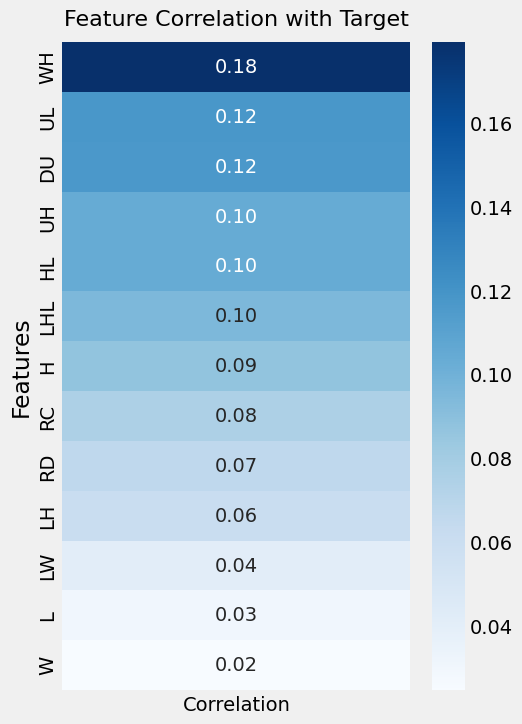
\includegraphics[width=0.4\textwidth]{figures/heatmap.png}
	\caption{Correlation heatmap of morphometric features with the sex of \textit{T. granosa}}
	\label{fig:heatmap}
\end{figure}

Exploratory data analysis was performed to characterize the dataset using visualizations to understand the patterns and correlations within the data. A correlation heatmap was created to assess the relationship between the predictors and the target variable.

The heatmap (see Figure~\ref{fig:heatmap}) revealed three features most correlated with the sex of \textit{T. granosa}: the width-height ratio (r = 0.18), the umbos-length ratio (r = 0.12), and the distance between the umbos (r = 0.12). Each of these features demonstrated a weak positive relationship with the target variable. 

\subsection{Statistical Analysis}

\begin{table}[H]
	\centering
	\small % or \footnotesize or \scriptsize
	\begin{tabular}{lc}
		\hline
		\textbf{Variable} & \textbf{p-value} \\ \hline
		Length & 0.334 \\
		Width & 0.753 \\
		Height & 0.124 \\
		Rib count & 0.251 \\
		Length (Hinge Line) & 0.120 \\
		Distance Umbos & 0.025 \\
		LW\_ratio & 0.011 \\
		LH\_ratio & 0.490 \\
		WH\_ratio & 0.003 \\
		UL\_ratio & 0.019 \\
		HL\_ratio & 0.079 \\
		UH\_ratio & 0.036 \\
		Rib Density & 0.181 \\ \hline
	\end{tabular}
	\caption{Mann-Whitney U Test Results for Sex-Based Feature Comparison}
	\label{tab:mann-whitney}
\end{table}

As part of the exploratory data analysis, statistical testing confirmed that the dataset did not follow a normal distribution. Consequently, the Mann-Whitney U test was applied with a significance level of $\alpha = 0.05$ to compare male and female samples. Out of thirteen features, five showed statistically significant differences. These included: distance between umbos ($p = 0.025$), length-width ratio ($p = 0.011$), umbos-length ratio ($p = 0.019$), width-height ratio ($p = 0.003$), and umbos-height ratio ($p = 0.036$). 

It is important to note that statistical significance does not imply predictive importance. Therefore, further analysis, such as feature importance evaluation, was performed to identify the most informative predictors for classification.

\subsection{Feature Importance Analysis}

\begin{figure}[!htbp]
	\centering
	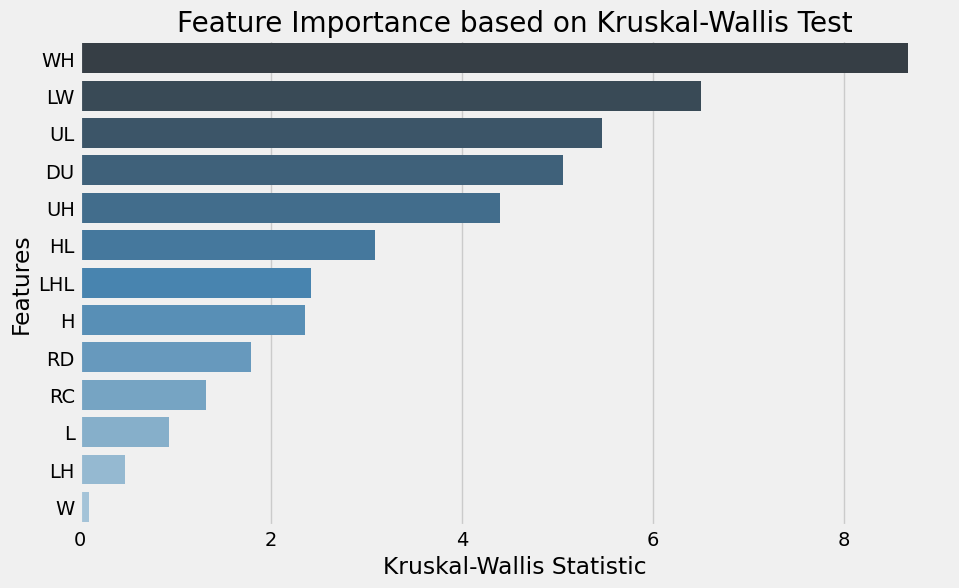
\includegraphics[width=1.0\textwidth]{figures/kw.png}
	\caption{Feature Importance Scores Using the Kruskal-Wallis Test}
	\label{fig:kw}
\end{figure}

Feature importance was assessed using the Kruskal-Wallis test, a non-parametric method that is suitable for evaluating differences in distributions across groups when the data does not follow a normal distribution. This approach was chosen because of the non-normality of the dataset and its robustness in handling continuous and ordinal data without assuming homogeneity of variances. \cite{ribeiro2024}

The analysis showed that the width-to-height ratio (WH\_ratio) had the highest importance score, indicating it is the most statistically significant feature for distinguishing the sex of \textit{T. granosa}. Other notable features included the length-to-width ratio (LW\_ratio), umbos-to-length ratio (UL\_ratio), and the distance between the umbos, all of which contributed significantly to the classification task.

\subsection{Performance Evaluation}

\begin{table}[H]
	\centering
	\resizebox{\textwidth}{!}{
		\begin{tabular}{lcccccc}
			\hline
			\textbf{Model} & \textbf{Accuracy (\%)} & \textbf{Precision (\%)} & \textbf{Recall (\%)} & \textbf{F1-Score (\%)} \\ \hline
			Support Vector Machine   & 58.62 & 58.62 & 58.62 & 58.44 \\
			Logistic Regression      & 57.83 & 57.83 & 57.83 & 57.61 \\
			K-Nearest Neighbors      & 51.18 & 51.31 & 51.18 & 50.77 \\
			Extra Trees              & 60.24 & 56.98 & 56.69 & 56.39 \\
			Random Forest            & 59.07 & 59.46 & 59.06 & 58.74 \\
			Gradient Boosting        & 60.27 & 60.98 & 60.27 & 59.96 \\
			\cellcolor{celadon}AdaBoost & \cellcolor{celadon}60.63 & \cellcolor{celadon}60.98 & \cellcolor{celadon}60.63 & \cellcolor{celadon}60.39 \\
			\hline
		\end{tabular}
	}
	\caption{Performance Metrics for Models with All 13 Features}
	\label{tab:performance-13-features}
\end{table}

In table~\ref{tab:performance-13-features}, the performance of different machine learning models is presented using the full set of 13 features from the dataset. AdaBoost emerges as the highest-performing model, with an accuracy of 60.63\%, precision of 60.98\%, recall of 60.63\%, and an F1-score of 60.39\%. These results suggest that AdaBoost is particularly effective when utilizing all available features, likely due to its ability to combine multiple weak learners into a more robust model. 

\begin{table}[H]
	\centering
	\resizebox{\textwidth}{!}{
		\begin{tabular}{lcccccc}
			\hline
			\textbf{Model} & \textbf{Accuracy (\%)} & \textbf{Precision (\%)} & \textbf{Recall (\%)} & \textbf{F1-Score (\%)} \\ \hline
			Support Vector Machine   & 63.77 & 64.47 & 63.77 & 63.42 \\
			Logistic Regression      & 63.75 & 63.87 & 63.75 & 63.70 \\
			\cellcolor{celadon}K-Nearest Neighbors      & \cellcolor{celadon}64.16 & \cellcolor{celadon}64.97 & \cellcolor{celadon}64.16 & \cellcolor{celadon}63.75 \\
			Extra Trees              & 62.20 & 59.69 & 59.08 & 58.69 \\
			Random Forest            & 62.96 & 60.10 & 59.85 & 59.54 \\
			Gradient Boosting        & 63.39 & 64.24 & 64.16 & 64.04 \\
			AdaBoost                 & 61.02 & 61.26 & 61.02 & 60.82 \\
			\hline
		\end{tabular}
	}
	\caption{Performance Metrics for Models with 5 Features}
	\label{tab:performance-5-features}
\end{table}

Table~\ref{tab:performance-5-features} presents the performance of the same models using only the top 5 features identified through Kruskal-Wallis feature importance analysis. The top 5 features selected are distance between the umbos, length-to-width ratio, width-to-height ratio, umbos-to-height ratio and umbos-to-length ratio. 

Interestingly, the performance of the models improves with the reduced feature set. K-Nearest Neighbors (KNN) achieves the highest performance in this scenario, with an accuracy of 64.16\%, precision of 64.97\%, recall of 64.16\%, and an F1-score of 63.75\%. These results suggest that KNN benefits from using only the most significant features, showing a notable improvement over its performance when all 13 features are used. 